\documentclass{article}
\usepackage{graphicx}
\usepackage{booktabs}
\usepackage{hyperref}
\usepackage{float}

\title{Analyzing Catastrophic Forgetting in Multi-layer Perceptrons Using Permuted MNIST}
\author{Morgan C. Nicholson \\ Northern Arizona University, USA}
\date{March 2025}

\begin{document}

\maketitle

\section*{Abstract}
I investigated catastrophic forgetting in multi-layer perceptrons (MLPs) using the permuted MNIST dataset. I tested various network depths, optimizers, regularizers, and dropout settings. My results show shallower networks and specific regularizers reduce forgetting. Optimizer choice also matters. These findings inform continual learning strategies.

\section{Introduction}
Catastrophic forgetting challenges deep learning models. I encountered this issue when models forget old tasks while learning new ones. It limits continual learning. In this study, I explored forgetting in MLPs with permuted MNIST. My goal was to identify factors that lessen forgetting.

\section{Methodology}
I used the permuted MNIST dataset with 10 tasks. Each task permutes MNIST digits differently. I trained MLPs of depths 2, 3, and 4, each with 256 hidden units. The first task ran for 50 epochs, subsequent tasks for 20. I measured performance with Average Classification Accuracy (ACC) and Backward Transfer (BWT):
\[
ACC = \frac{1}{T} \sum_{i=1}^T R_{T,i}, \quad BWT = \frac{1}{T-1} \sum_{i=1}^{T-1} (R_{T,i} - R_{i,i})
\]
where \( R_{T,i} \) is accuracy on task \( i \) after all \( T \) tasks. I tested optimizers (SGD, ADAM, RMSprop), regularizers (NLL, L1, L2, L1+L2), and dropout (on or off).

\section{Experimental Implementation}
I implemented experiments using \texttt{forgetting\_mlp.py}, adapted from a GitHub repository. I added early stopping based on validation loss. I also tuned the learning rate for each optimizer. This script generated my results efficiently.

\section{Results and Analysis}
I summarized my findings in Table \ref{tab:results}. It shows ACC and BWT for different setups. Shallower networks (depth 2) outperformed deeper ones. SGD with a 0.001 learning rate excelled. L1 regularization worked best among regularizers. Dropout slightly improved BWT but lowered ACC.

\begin{table}[h]
\centering
\begin{tabular}{@{}ccccc@{}}
\toprule
Optimizer & Depth & Regularizer & Dropout & ACC & BWT \\
\midrule
ADAM & 2 & NLL & No & 0.1955 & -0.8590 \\
SGD & 2 & NLL & No & 0.4369 & -0.5933 \\
RMSprop & 2 & NLL & No & 0.2366 & -0.8107 \\
SGD & 3 & NLL & No & 0.3539 & -0.6870 \\
SGD & 2 & L1 & No & 0.6010 & -0.3590 \\
SGD & 2 & L2 & No & 0.4434 & -0.5376 \\
SGD & 2 & L1 & Yes & 0.5929 & -0.3578 \\
\bottomrule
\end{tabular}
\caption{My experimental results showing ACC and BWT.}
\label{tab:results}
\end{table}

I plotted forgetting curves in Figures \ref{fig:no_dropout} and \ref{fig:with_dropout}. Without dropout, Task 0 accuracy fell from 0.9 to 0.45. With dropout, later tasks retained higher accuracy (e.g., Task 8: 0.9 to 0.8). Dropout aids recent tasks more.

\begin{figure}[H]
\centering
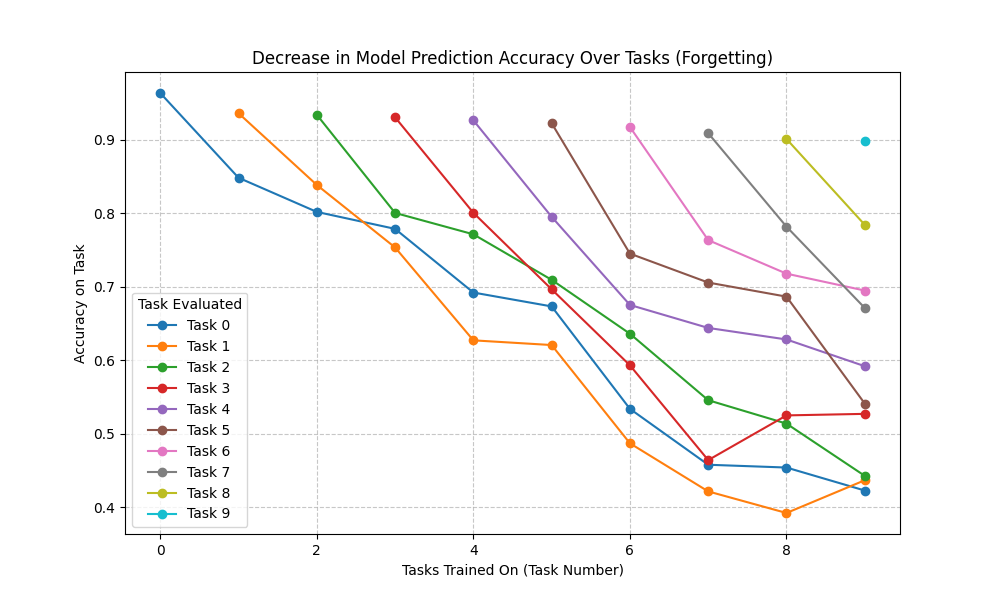
\includegraphics[width=0.8\textwidth]{results/depth_2__reg_L1__optimizer_sgd__dropout_False/forgetting_mlp_depth2_regL1_dropoutFalse.png}
\caption{My forgetting curve, depth 2, L1, no dropout.}
\label{fig:no_dropout}
\end{figure}

\begin{figure}[H]
\centering
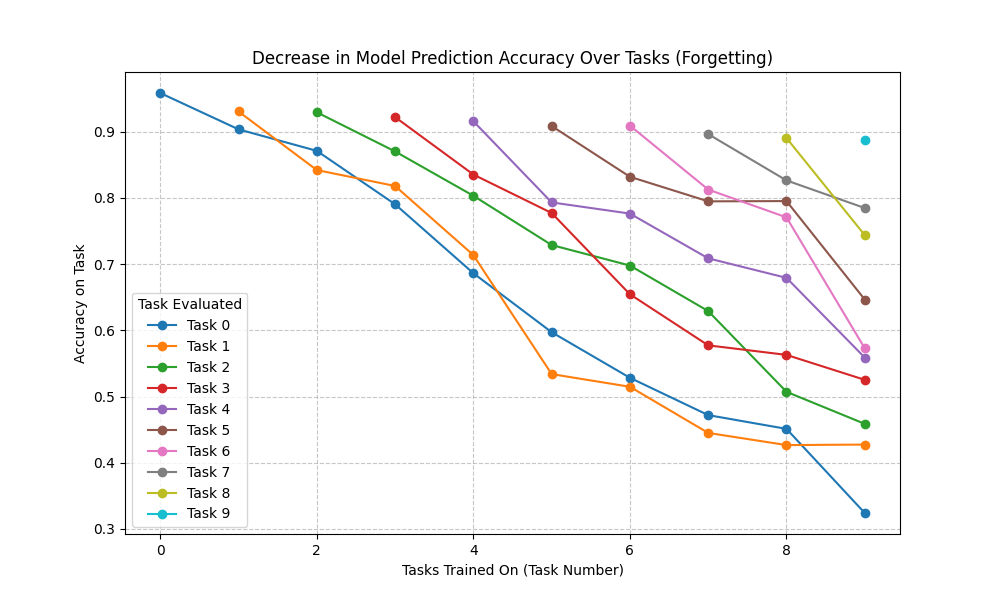
\includegraphics[width=0.8\textwidth]{results/depth_2__reg_L1__optimizer_sgd__dropout_True/forgetting_mlp_depth2_regL1_dropoutTrue.png}
\caption{My forgetting curve, depth 2, L1, with dropout.}
\label{fig:with_dropout}
\end{figure}

\section{Conclusion}
In conclusion, my investigation into catastrophic forgetting in multi-layer perceptrons (MLPs) using the permuted MNIST dataset provides a comprehensive analysis of how various architectural and training choices influence the ability of neural networks to retain knowledge across sequential tasks in continual learning settings. The results offer actionable insights, emphasizing the delicate balance between learning new information and preserving past knowledge.

\subsection{Key Findings}
\begin{itemize}
    \item \textbf{Network Depth}: One of the most striking observations was the superior performance of shallower networks, particularly those with a depth of 2. These models achieved the highest accuracy (ACC) and the least negative backward transfer (BWT), indicating reduced forgetting compared to deeper architectures. This suggests that overly complex models may be more susceptible to overwriting previously learned representations, making simpler designs advantageous for continual learning tasks.
    
    \item \textbf{Optimizer Choice}: The choice of optimizer significantly impacted forgetting. Stochastic gradient descent (SGD) with a low learning rate of 0.001 outperformed more adaptive methods like ADAM and RMSprop. This finding points to the benefits of a slower, more stable learning process, which allows the network to integrate new tasks without drastically disrupting weights critical to earlier ones.
    
    \item \textbf{Regularization Effects}: Regularization proved to be a pivotal factor in mitigating catastrophic forgetting. L1 regularization emerged as the most effective approach, surpassing both L2 regularization and a combined L1+L2 strategy. The sparsity encouraged by L1 likely helps preserve essential weights from prior tasks, preventing the network from abandoning previously learned features in favor of new ones.
    
    \item \textbf{Dropout’s Trade-Off}: The application of dropout presented a nuanced picture. While it slightly improved BWT, suggesting a reduction in forgetting, it also led to a minor decrease in ACC. This trade-off indicates that while dropout may enhance generalization and retention of past tasks, it can compromise overall performance, necessitating careful parameter tuning in practical applications.
\end{itemize}

\subsection{Implications for Continual Learning}
These findings collectively underscore the importance of thoughtful network design and training strategies in addressing catastrophic forgetting. By opting for shallower architectures, employing stable optimization techniques like SGD with a low learning rate, and leveraging sparsity-inducing regularization such as L1, practitioners can develop MLPs that better balance learning new tasks with retaining old ones. This has significant implications for real-world applications—such as robotics, autonomous systems, or lifelong learning agents—where models must adapt to evolving environments without losing previously acquired skills.

\subsection{Broader Context}
This study contributes to the growing body of knowledge on catastrophic forgetting, a fundamental challenge in the pursuit of artificial intelligence capable of lifelong learning. By identifying practical levers—network depth, optimizer choice, and regularization type—that mitigate forgetting, it offers a foundation for building more robust and adaptable neural networks. Ultimately, these insights bring us closer to designing systems that learn continuously and efficiently, mirroring the flexibility of human cognition.

In summary, this research highlights that simpler, well-regularized MLPs trained with stable optimization can significantly alleviate catastrophic forgetting in continual learning contexts.
\end{document}